% !TEX root = ../paper.tex
%http://sphweb.bumc.bu.edu/otlt/MPH-Modules/BS/BS704_HypothesisTesting-ANOVA/BS704_HypothesisTesting-Anova_print.html
\section{Results}\label{sec:results}
Some data points needed to be removed from the experiments, in order to gain a clearer understanding of the data we gathered. 

From the \target, we started with a total of 7344 attempts.
176 were removed because of system errors, were the system wrongly activated a technique attempt even though the user did not intend to do so.
Another 406 attempts were removed as outliers using the Outlier Labeling method described by Hoaglin and Iglewicz in Resistant Rules for Outlier Labeling \cite{Hoaglin:1987}.
This gave us a total of 6762 attempts for the \target.

From the \accuracy, we started with a total of 4752 attempts.
111 attempts were removed to system errors. 
Finally 130 attempts were removed with the same Outlier Labeling method used above.
This gave us a total of 4511 attempts for the \accuracy.

\subsection{Success rate}
The results presented here will be based on the data collected during the \target. 
Here we will be presenting results relating to whether or not the user hit the target, which we will be referring to as effectiveness when discussing the results. 

To see whether or not each technique had an effect on the effectiveness of each attempt, we performed a Pearsons Chi-Square test on both data sets. 
For the \push techniques, $X(3)=121.950$, $p<0.001$, and for the \pull techniques we got $X(3)=438.473$, $p<0.001$. 
This means that both \push and \pull techniques had a significant effect on the effectiveness of each attempt. 
\Cref{tab:successRate} shows the success rate for each of the techniques. 

\begin{table}[H]
	\centering
		\begin{tabular}{c c c c c}
			\cline{2-5}
			& \multicolumn{4}{c}{\textbf{Hit Success Means}} \\
			\cline{2-5}
			& \textbf{Grab} & \textbf{Swipe} & \textbf{Throw} & \textbf{Tilt} \\ \hline
			\textbf{Push} & 95.9\% & 96\% & 93.2\% & 83.3\% \\ \hline
			\textbf{Pull} & 94\% & 97.5\% & 96.7\% & 71.8\% \\ \hline
		\end{tabular}
	\caption{Success rate for each technique}
	\label{tab:successRate}
\end{table}

\subsection{Time taken}
This section will be presenting results based on the \target.
Here, we will be presenting the results in regards to how long each user took in performing each technique. 
When discussing these results, we will be referring to them as a techniques efficiency.

We performed a linear mixed effects model analysis on the data to see if how time was affected by the different aspects of our experiment. 
We found out that effectiveness had no effect on the time each user took per attempt ($F_{1,6706.785} = 2.283, p = 0.131$), and neither had the direction of the technique ($F_{1,6695.822} = 1.952, p = 0.162$). 
The target size ($F_{1,6695.228} = 91.634, p < 0.001$) and the technique  ($F_{1,6695.228} = 91.634, p < 0.001$) though did have significant effects on the time taken per attempt. 
We performed a post-hoc LSD pairwise comparison on the techniques to see how each technique differed from one another and found that all techniques were significantly different $(p<0.001)$ from each other. 

We also found that there were other interactions between the variables that were affecting the time for each attempt differently. 
$Direction \times Technique$  ($F_{3,6694.657} = 52.272, p < 0.001$), $Effectiveness \times Technique$  ($F_{3,6696.169} = 5.227, p < 0.001$) and finally $Effectiveness \times Direction \times Technique$  ($F_{3,6696.038} = 10.235, p < 0.001$) all showed to be significant interactions. 
We then ran another post-hoc LSD pairwise test between successful and failed techniques for each technique and direction to see were that significance was. 
The only significantly different pair was between \grab \push and \pull $(p < 0.001)$.

Below you can find the means for each technique and direction in table something
\todo[inline]{add table}

\subsection{Distance from target}
The data that was used to measure the distance from the target was based on the \accuracy experiment.
Here we will present the results in regards to how far away from the center of the target (in pixels) each user was when performing the technique. 
This will be referred as a a techniques accuracy when we discuss the results presented in this section. 

We performed another linear mixed effects model analysis on the data to see if each technique had a significant effect on the accuracy of each attempt. 

%!TEX root = ../paper.tex
\begin{figure}[H]
\centering
%\textbf{Time performance means}\\[4pt]
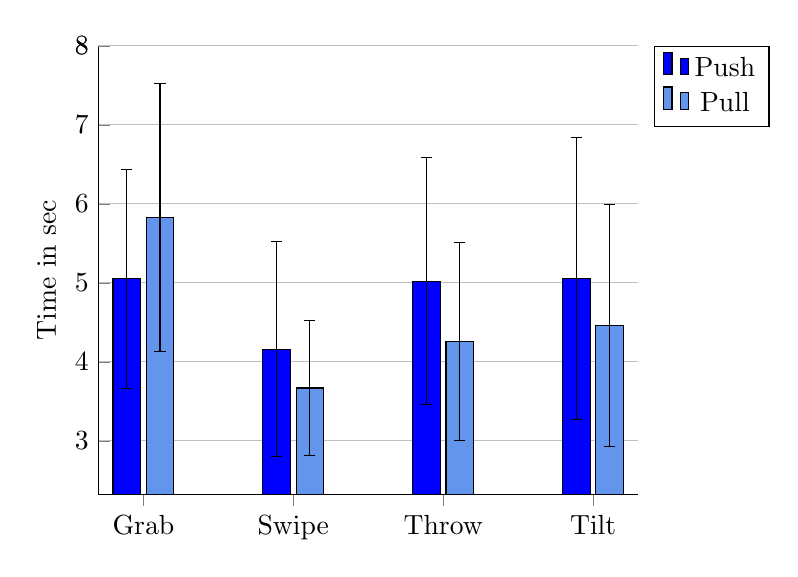
\begin{tikzpicture}
\begin{axis}[
    ybar,
    legend pos = outer north east,
    ylabel={Time in sec},
    %xlabel={Technique},
    symbolic x coords={Grab,Swipe,Throw,Tilt},
    xtick=data,
    axis lines*=left,
    ymajorgrids,
    extra y ticks=8,
    extra y tick style={grid=none},
    ytick={1,...,8}
    ]
\addplot[fill=blue] plot[error bars/.cd, y dir=both, y explicit] coordinates {
    (Grab,5.05) +- (1.385,1.385)
    (Swipe,4.16) +- (1.361,1.361) 
    (Throw,5.02) +- (1.565,1.565)
    (Tilt,5.06) +- (1.785,1.785)
    };
\addplot[fill=CornflowerBlue] plot[error bars/.cd, y dir=both, y explicit] coordinates {
    (Grab,5.83) +- (1.697,1.697)
    (Swipe,3.67) +- (0.859,0.859) 
    (Throw,4.26) +- (1.254,1.254)
    (Tilt,4.46) +- (1.532,1.532)
    };
\legend{Push,Pull}
\end{axis}
\end{tikzpicture}
\caption{The time means for each technique.}
\end{figure}

% \begin{tikzpicture}
%\pgfplotsset{symbolic x coords={Grab,Swipe,Throw,Tilt}, ymin=0, ymax=19, ybar stacked, ylabel={Time in sec}, xtick=data}
%\begin{axis}[bar shift=-8pt,
%    legend pos = outer north east, legend style = {name = serieA}, reverse legend]
%    \addplot[black, fill=CornflowerBlue, postaction={pattern=north east lines}] plot[error bars/.cd, y dir=both, y explicit] coordinates {
%    (Grab,4.81) +- (1.307,1.307)
%    (Swipe,3.83) +- (1.236,1.236) 
%    (Throw,4.72) +- (1.504,1.504)
%    (Tilt,4.66) +- (1.652,1.652)
%    };
%    \addplot[fill=CornflowerBlue] plot[error bars/.cd, y dir=both, y explicit] coordinates {
%    (Grab,5.3) +- (1.421,1.421)
%    (Swipe,4.5) +- (1.399,1.399) 
%    (Throw,5.33) +- (1.565,1.565)
%    (Tilt,5.48) +- (1.825,1.825)
%    };
%    \addplot[fill=CornflowerBlue] plot[error bars/.cd, y dir=both, y explicit] coordinates {
%    (Grab,5.05) +- (1.385,1.385)
%    (Swipe,4.16) +- (1.361,1.361) 
%    (Throw,5.02) +- (1.565,1.565)
%    (Tilt,5.06) +- (1.785,1.785)
%    };
%    \legend{Push (large), Push (small), Push (total)}
%  \end{axis}
%  \begin{axis}[bar shift = 8pt,
%  legend style = {at = {([yshift = -4.5mm, xshift = -4.5mm]serieA.south west)},
%      anchor = north west}, reverse legend]
%    \addplot[black, fill=blue, postaction={pattern=north east lines}] plot[error bars/.cd, y dir=both, y explicit] coordinates {
%    (Grab,5.46) +- (1.474,1.474)
%    (Swipe,3.42) +- (1.474,1.474) 
%    (Throw,4.02) +- (1.256,1.256)
%    (Tilt,4.18) +- (1.411,1.411)
%    };
%    \addplot[fill=blue] plot[error bars/.cd, y dir=both, y explicit] coordinates {
%    (Grab,6.19) +- (1.824,1.824)
%    (Swipe,3.92) +- (0.858,0.858) 
%    (Throw,4.51) +- (1.206,1.206)
%    (Tilt,4.76) +- (1.6,1.6)
%    };
%    \addplot[fill=CornflowerBlue] plot[error bars/.cd, y dir=both, y explicit] coordinates {
%    (Grab,5.83) +- (1.697,1.697)
%    (Swipe,3.67) +- (0.859,0.859) 
%    (Throw,4.26) +- (1.254,1.254)
%    (Tilt,4.46) +- (1.532,1.532)
%    };
%    \legend{Pull (large), Pull (small), Pull (total)}
%  \end{axis}
% \end{tikzpicture}

